\documentclass[../../main.tex]{subfiles}


\begin{document}
\subsection*{(a)}
We use the Plugin 'Filter Log on Trace Attribute Values' to only select Tickets of type 'Task'. As visualization, we then choose 'Explore Event Log'.
This gives us the table below:\\
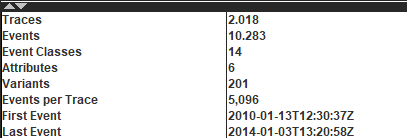
\includegraphics[width=0.5\columnwidth]{img/ProM_a_traces.png}\\
From it, we can take that there are 2018 traces, 201 trace variants and 10283 events. We then apply the plugin 'Mine Petri net with Inductive Miner' on this filtered log and make sure we choose 'Inductive Miner - Infrequent (IMf)' as our variant and set it to 20\% by assigning the Noise threshold to 0.20. This results in the following Model:\\
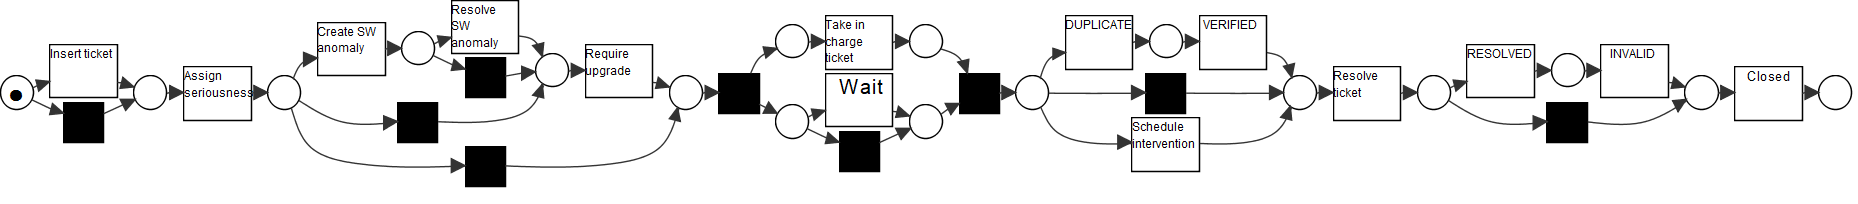
\includegraphics[width=\columnwidth]{img/ProM_a_inductive_miner.png}

\subsection*{(b)}
We use the plugin 'Multi-perspective Process Explorer' on our Petri net from (a). This gives us the following information on fitness and precision:\\
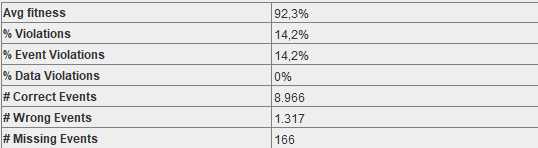
\includegraphics[width=0.5\columnwidth]{img/ProM_b_fitness.png}
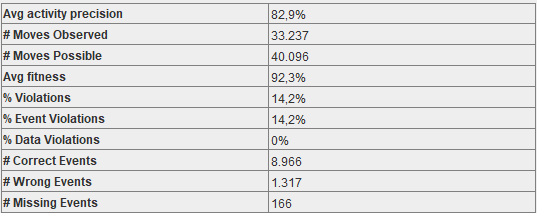
\includegraphics[width=0.5\columnwidth]{img/ProM_b_precision.png}\\
We obtain the percentage of fitting traces by calculating 100\% minus the percentage of violations (100\% - 14.2\%), resulting in 85,8\% fitting traces. Alignment-based fitness (92.3\%) and precision (82.9\%) can be read from the tables above.\\
By using the inductive miner again and adjusting the infrequency parameter to 10\% we obtain a process model with better fitness, precision and more perfectly fitting traces than before. The stats of the new model can be seen below:\\
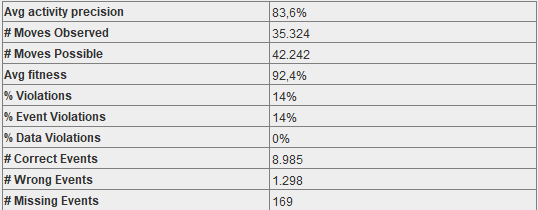
\includegraphics[width=0.5\columnwidth]{img/ProM_b_model_2.png}

\subsection*{(c)}
We used the plugin 'Align Log and Model for Repair (global costs)' for this subtask. We used the default values.
\subsubsection*{Move on Model}
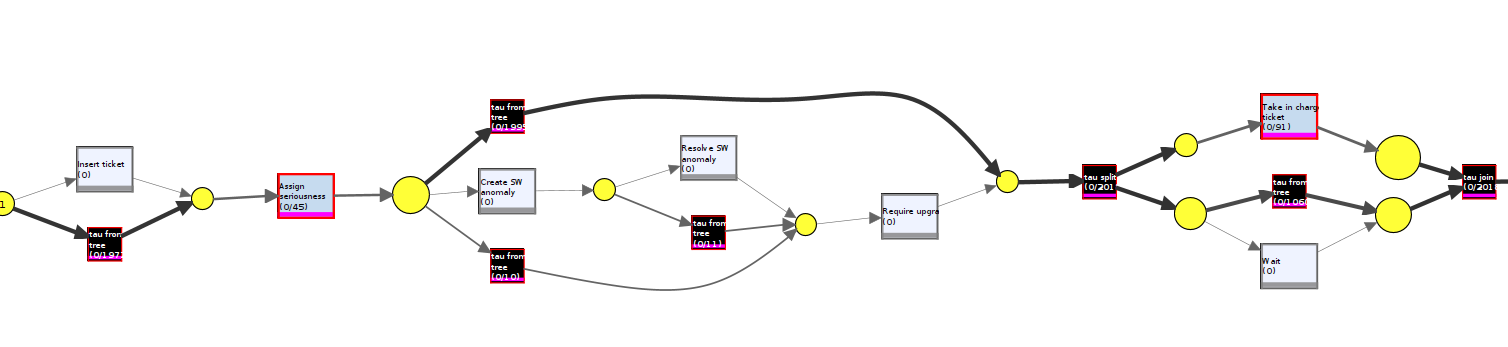
\includegraphics[width=\columnwidth]{img/ProM_c_Move_on_Model.png} \\
Moves on Model occur obviously at every hidden transition (since they aren't in the log) and the activities of 'Assign seriousness', 'Take in charge ticket', 'Resolve ticket', 'Closed'. The later two just have fairly few moves on logs and are acceptable in the model, since there are cases with tickets still in progress in the log. \\
The first two activities are important for improving the model or even the ticketing system. We see that not every case executes Assign seriousness. Perhaps this transition should be skipable by a tau-transition. However, the assignment introduction states that either 'Insert ticket' or 'Assign seriousness' should be executed first. Therefore, the model could also have an option between both in the beginning, instead of putting one behind the other. \\
That 'Take in charge ticket' was moved on the model 91 times should also be noted. That the model set this action in parallel with 'Wait' seems problematic. It should be possible to wait any time in the ticketing process in order to execute some activity later on.

\subsubsection*{Move on Log}
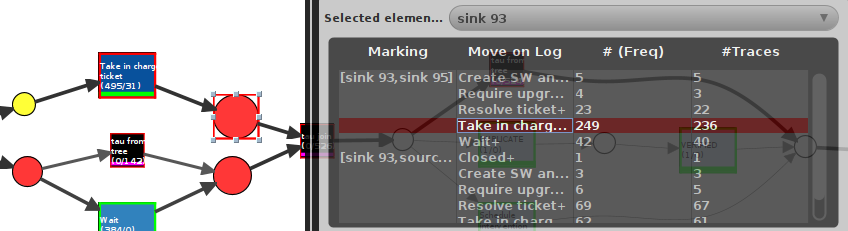
\includegraphics[width=\columnwidth]{img/ProM_c_Move_on_Log_1.png} \\
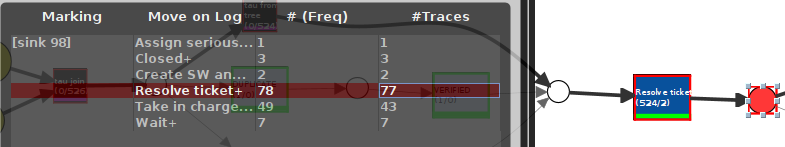
\includegraphics[width=\columnwidth]{img/ProM_c_Move_on_Log_2.png} \\
We can analyze Moves on Logs by clicking on the big places in the visualization. As one can see, the transitions 'Take in charge ticket' and 'Resolve ticket' experience the most moves on log in the model. We used the Movement Container Filter to only allow traces with moves on logs in these transitions.

\end{document}